

\documentclass[12pt]{article}
\usepackage[margin=1in]{geometry}
\setlength{\emergencystretch}{1em}
\usepackage{amsmath, amssymb, amsthm}
\usepackage{graphicx}
\usepackage{xcolor}
\usepackage{listings}
\usepackage{caption}
\usepackage{natbib}
\usepackage{xr}
\usepackage[hidelinks]{hyperref}
\usepackage{placeins}
\usepackage{float}
\usepackage{pdflscape}
\usepackage{booktabs}
\usepackage{algorithm}
\usepackage{algpseudocode}
\usepackage{subcaption}
\usepackage{multirow}
\usepackage{tikz}
\usetikzlibrary{arrows.meta, positioning}
\DeclareMathOperator{\Var}{Var}
\DeclareMathOperator{\Cov}{Cov}
\newcommand{\E}{\mathbb{E}}
\newcommand\independent{\protect\mathpalette{\protect\independenT}{\perp}}
\def\independenT#1#2{\mathrel{\rlap{$#1#2$}\mkern2mu{#1#2}}}

% ---- switches ---------------------------------------------------------------
\newif\iffixnotes  \fixnotesfalse    % \fixnotesfalse -> clean submission build

\newcommand{\FIX}[2]{%
  \iffixnotes
    \par\smallskip\noindent
    \fcolorbox{orange!50}{orange!7}{%
      \parbox{0.95\linewidth}{\footnotesize\sffamily\color{orange!35!black}%
        \textbf{[#1]\ }#2}}%
    \par\smallskip
  \fi}


\externaldocument[][nocite]{methodology-8.3.5}
\renewcommand{\thesection}{S\arabic{section}}
\renewcommand{\thetable}{S\arabic{table}}
\renewcommand{\thefigure}{S\arabic{figure}}
\renewcommand{\theequation}{S\arabic{equation}}
\renewcommand{\thealgorithm}{S\arabic{algorithm}}

% Changed text is blue when compiled through the highlighted review wrapper.
\definecolor{revisionblue}{RGB}{0,76,170}
\newcommand{\rev}[1]{\ifdefined\ReviewChanges{\color{revisionblue}#1}\else#1\fi}
\pdfstringdefDisableCommands{\def\rev#1{#1}}

\begin{document}
\title{Supplementary Material\\\rev{SP-BART}: A Semi-parametric BART for estimating heterogeneous treatment effects}
\author{Yusufhan Balci, Mark van de Wiel and Jeroen Hoogland}
\date{Version 8.3.5}
\maketitle
\label{SEC:supplement}
\noindent This supplement provides additional simulation and application results and computational details.


\section{Orthogonalisation of the Treatment Contrast}
\label{subsec:ortho_supp}

The standard fit uses centered treatment coding, $z-0.5$. In the orthogonalised fit, we use $z-\hat\pi(x)$ instead. We estimate $\hat\pi(x)$ once with a Bayesian logistic regression \rev{including main effects and pairwise interactions}, and hold it fixed across chains. \rev{Both fits use the same prognostic forest specification and prior. Residualising treatment changes the conditional outcome function represented by the prognostic component.}

In this comparison, orthogonalising the treatment contrast increases CATE RMSE in every design, by $12.6$ to $37.2\%$ (Table~\ref{tab:ortho}). Under a linear $\mu$, the increase averages $17.1\%$, with wider intervals and similar coverage. Under a non-linear $\mu$, the increase averages $29.4\%$ and coverage falls despite wider intervals. The last two columns of Table~\ref{tab:ortho} use the same interval-based top-quartile rule as in the main simulations; sensitivity falls in both panels.

The standard-arm values come from this separate experiment and differ from those in main-text Table \ref{tab:default_scenario}. There are 200 replicates at each sample size.

\begin{table}[htbp]
\centering\small
\caption{Orthogonalised versus standard \rev{SP-BART} under both prognostic forms, with 200 replicates per setting. Change is the percentage increase in CATE RMSE. Sensitivity uses the same interval-based top-quartile rule as in the main simulations.}
\label{tab:ortho}
\resizebox{\textwidth}{!}{%
\begin{tabular}{rccccccccc}
\toprule
& \multicolumn{3}{c}{CATE RMSE} & \multicolumn{2}{c}{Coverage} & \multicolumn{2}{c}{CI width} & \multicolumn{2}{c}{Top-25\% sensitivity}\\
\cmidrule(lr){2-4}\cmidrule(lr){5-6}\cmidrule(lr){7-8}\cmidrule(lr){9-10}
$N$ & standard & residualised & change & standard & residualised & standard & residualised & standard & residualised\\
\midrule
\multicolumn{10}{l}{\emph{Linear $\mu$}}\\
250 & 0.639 & 0.800 & $+25.1\%$ & 0.942 & 0.957 & 2.415 & 3.253 & 0.491 & 0.376 \\
500 & 0.381 & 0.454 & $+19.1\%$ & 0.959 & 0.965 & 1.619 & 1.945 & 0.621 & 0.551 \\
750 & 0.312 & 0.355 & $+13.5\%$ & 0.963 & 0.966 & 1.307 & 1.512 & 0.689 & 0.637 \\
1000 & 0.260 & 0.304 & $+16.7\%$ & 0.965 & 0.966 & 1.116 & 1.287 & 0.732 & 0.686 \\
1500 & 0.205 & 0.237 & $+15.8\%$ & 0.969 & 0.968 & 0.900 & 1.021 & 0.776 & 0.743 \\
3000 & 0.143 & 0.161 & $+12.6\%$ & 0.967 & 0.968 & 0.623 & 0.697 & 0.843 & 0.823 \\
\midrule
\multicolumn{10}{l}{\emph{Non-linear $\mu$}}\\
250 & 0.578 & 0.737 & $+27.5\%$ & 0.957 & 0.955 & 2.318 & 2.970 & 0.465 & 0.402 \\
500 & 0.350 & 0.481 & $+37.2\%$ & 0.968 & 0.956 & 1.532 & 1.908 & 0.612 & 0.558 \\
750 & 0.266 & 0.346 & $+30.1\%$ & 0.977 & 0.971 & 1.219 & 1.477 & 0.676 & 0.623 \\
1000 & 0.223 & 0.295 & $+32.4\%$ & 0.978 & 0.969 & 1.037 & 1.254 & 0.717 & 0.659 \\
1500 & 0.176 & 0.223 & $+26.5\%$ & 0.978 & 0.973 & 0.828 & 0.989 & 0.776 & 0.737 \\
3000 & 0.123 & 0.152 & $+23.0\%$ & 0.979 & 0.976 & 0.574 & 0.677 & 0.841 & 0.812 \\
\bottomrule
\end{tabular}}
\end{table}

\section{Homogeneous Simulation Results}
Table \ref{tab:hom_scenario} presents the results for the homogeneous simulation scenario, where $\tau(x)=3$ and all non-intercept treatment-effect coefficients are zero. The results show that \rev{SP-BART and BCF perform similarly and can shrink back towards homogeneity}.


\begin{table}[htbp]
\centering
\caption{Performance Comparison in the \textbf{Homogeneous Scenario} (Constant CATE, $\tau=3$). Results are shown for models with Homogeneous Treatment Effects, comparing Linear and Non-linear prognostic functions ($\mu$).}
\label{tab:hom_scenario}
\resizebox{\textwidth}{!}{
\begin{tabular}{lr ccc ccc c ccc ccc}
\toprule
& & \multicolumn{6}{c}{\textbf{BCF}} & & \multicolumn{6}{c}{\textbf{\rev{SP-BART}}} \\
\cmidrule{3-8} \cmidrule{10-15}
$\mu(x)$ Form & $N$ & \multicolumn{3}{c}{ATE} & \multicolumn{3}{c}{CATE} & & \multicolumn{3}{c}{ATE} & \multicolumn{3}{c}{CATE} \\
\cmidrule{3-5} \cmidrule{6-8} \cmidrule{10-12} \cmidrule{13-15}
& & RMSE & Cov & Len & RMSE & Cov & Len & & RMSE & Cov & Len & RMSE & Cov & Len \\
\midrule
\multirow{6}{*}{Linear}
& 250 & 0.326 & 0.82 & 0.852 & 0.494 & 0.96 & 2.039 &  & 0.348 & 0.80 & 0.859 & 0.590 & 0.94 & 2.268 \\
& 500 & 0.193 & 0.84 & 0.559 & 0.337 & 0.97 & 1.445 &  & 0.198 & 0.83 & 0.557 & 0.347 & 0.96 & 1.501 \\
& 750 & 0.150 & 0.88 & 0.442 & 0.275 & 0.98 & 1.179 &  & 0.153 & 0.85 & 0.441 & 0.284 & 0.96 & 1.216 \\
& 1000 & 0.136 & 0.81 & 0.377 & 0.243 & 0.98 & 1.018 &  & 0.137 & 0.81 & 0.376 & 0.238 & 0.97 & 1.036 \\
& 1500 & 0.100 & 0.86 & 0.303 & 0.201 & 0.98 & 0.827 &  & 0.101 & 0.84 & 0.303 & 0.187 & 0.97 & 0.836 \\
& 3000 & 0.069 & 0.89 & 0.210 & 0.142 & 0.97 & 0.569 &  & 0.068 & 0.89 & 0.211 & 0.132 & 0.96 & 0.576 \\
\midrule
\multirow{6}{*}{Non-linear}
& 250 & 0.247 & 0.93 & 0.825 & 0.470 & 0.97 & 1.934 &  & 0.250 & 0.92 & 0.810 & 0.549 & 0.95 & 2.188 \\
& 500 & 0.159 & 0.91 & 0.535 & 0.314 & 0.97 & 1.303 &  & 0.162 & 0.92 & 0.530 & 0.331 & 0.96 & 1.445 \\
& 750 & 0.109 & 0.94 & 0.424 & 0.235 & 0.99 & 1.068 &  & 0.109 & 0.96 & 0.422 & 0.248 & 0.98 & 1.150 \\
& 1000 & 0.089 & 0.95 & 0.363 & 0.207 & 0.98 & 0.938 &  & 0.090 & 0.95 & 0.360 & 0.205 & 0.98 & 0.981 \\
& 1500 & 0.080 & 0.93 & 0.291 & 0.175 & 0.98 & 0.761 &  & 0.080 & 0.91 & 0.288 & 0.166 & 0.97 & 0.782 \\
& 3000 & 0.051 & 0.95 & 0.201 & 0.124 & 0.99 & 0.530 &  & 0.049 & 0.96 & 0.200 & 0.115 & 0.98 & 0.545 \\
\bottomrule
\end{tabular}}
\end{table}

\section{Coverage-matched Individual CATE Inference on IHDP}
\label{subsec:ihdp_matched_supp}

This calibration is possible because the individual treatment effects are known in the semi-synthetic benchmark.

The original $95\%$ credible intervals of the two Bayesian methods do not have the same coverage of the true $\tau_i$ on IHDP, so their exclusion rates are not directly comparable. Let $m_i$ be the posterior mean, and $q_{i,0.025}$ and $q_{i,0.975}$ the posterior percentiles that form the central $95\%$ credible interval. We rescale this interval as
\[
 I_i(c)=\left[m_i+c\{q_{i,0.025}-m_i\},\;m_i+c\{q_{i,0.975}-m_i\}\right].
\]
The scale factor $c>1$ widens the interval. For each held-out replicate and each model, we choose the smallest $c$ attaining at least $95\%$ empirical coverage across the other 99 data sets, and then evaluate it on the held-out replicate. The resulting intervals are empirically calibrated CATE intervals, not tolerance intervals or necessarily $95\%$ posterior credible intervals. The shared covariates and treatment assignments mean this evaluates calibration across IHDP response surfaces rather than across new patient samples. Table~\ref{tab:ihdp_posterior_matched} reports the comparison; held-out mean coverage is $0.950$ for both methods. The exclusion rates are close.

\begin{table}[htbp]
\centering\footnotesize
\caption{Coverage-matched individual CATE inference on IHDP. Each model's
intervals are rescaled towards a common empirical coverage target of $95\%$. The scale
factor is chosen from the other 99 data sets and then applied to the held-out
one; held-out coverage need not equal the target exactly. Values are mean (standard error) over 100 replicates. The scale factor
$c$ multiplies the distances from the posterior mean to the $2.5$th and $97.5$th posterior percentiles; $c>1$ widens the interval. ``Correct exclusion'' is the fraction
of children whose interval excludes zero in the direction of the true effect.}
\label{tab:ihdp_posterior_matched}
\resizebox{\textwidth}{!}{%
\begin{tabular}{lcccccc}
\toprule
Method & $c$ & coverage & excludes $0$ & correct exclusion & Type S & width\\
\midrule
\textbf{\rev{SP-BART}} & 1.105 (0.000) & 0.950 (0.004) & 0.876 (0.008) & 0.875 (0.008) & 0.001 (0.000) & 5.56 (0.61)\\
BCF & 1.186 (0.000) & 0.950 (0.003) & 0.878 (0.010) & 0.876 (0.010) & 0.002 (0.000) & 5.39 (0.76)\\
\bottomrule
\end{tabular}}
\end{table}

\section{Detailed Analysis: The CANVAS Program}
\label{SEC:supplement_canvas}

\subsection{Out-of-Sample Performance}
\label{subsec:oos_performance}

We compare \rev{SP-BART} with BCF by using an analytic sample of 5018 individuals from CANVAS-R for training and 3004 individuals from CANVAS for validation. These are the numbers included in this analysis, rather than the original trial enrolments. To study the effect of sample size, we drew 20 treatment-stratified samples without replacement for $N \in \{500, 1000, 1500, 2000, 3000, 4000\}$ from CANVAS-R and trained both models on each sample. We also fit both models once on the full CANVAS-R sample. \rev{Both models include the treatment proportion in the full CANVAS-R training pool as the same constant propensity score in the prognostic component.} We evaluate agreement between the models using the correlation between their out-of-sample CATEs, and we evaluate ranking using the uplift curve \citep{rzepakowski2010decision}. Because the outcome is follow-up minus baseline HbA1c, a more negative CATE indicates greater benefit. The uplift curve ranks individuals from high to low predicted benefit, $-\hat\tau(x)$, and plots the cumulative gain as an increasing portion of the population is treated. This evaluation relies on randomization; without exchangeability, the empirical treatment effect cannot be compared directly with the model output. Figure \ref{fig:cv_dashboards} and Table \ref{tab:model_metrics} show the results for both methods at the different sample sizes.

The comparison of the individual CATEs shows that the two models already agree reasonably well at small $N$, and that this agreement increases with sample size (Table \ref{tab:model_metrics} and Figure \ref{fig:cv_dashboards}). At $N=1000$ the average correlation of the out-of-sample CATEs is $r = 0.69$; at $N=4000$ it is $r = 0.81$, and $r = 0.84$ when both models are trained on the whole CANVAS-R sample. Spearman correlations are similar. This indicates similar estimated treatment effect patterns, although agreement between models does not establish the true functional form. At smaller sample sizes, both models often shrink the treatment effect back towards homogeneity, BCF more strongly.

The uplift curves in Figure \ref{fig:cv_dashboards} are comparable for both models and remain close to the diagonal representing random targeting. This limits the evidence for improved targeting despite agreement between the models. The normalized net areas under the uplift curve in Table \ref{tab:model_metrics} are similar as well. Thus, even when the CATE magnitudes differ at lower sample sizes, the models rank patients similarly. \rev{SP-BART} also has smaller RMSEs for the out-of-sample outcome ($Y$) at every training size in Table \ref{tab:model_metrics}. In this evaluation, \rev{SP-BART} therefore provides comparable ranking while also allowing direct variable selection, which we examine in the next section.

To standardize the area under the uplift curve, write $U(f)$ for cumulative uplift when the fraction $f$ of the validation sample is selected. With $n_v=3004$, we report
\[
 \frac{\operatorname{NetAUUC}}{n_v}
 =\frac{1}{n_v}\left\{\int_0^1 U(f)\,df-\frac{U(1)}{2}\right\}.
\]
We subtract the area under the straight line for random targeting and divide by the validation-sample size. Positive values indicate greater cumulative HbA1c reduction than random targeting. Table \ref{tab:model_metrics} reports this normalized measure.

At $N=500$, the outcome-RMSE standard deviation is much lower for \rev{SP-BART} than for BCF ($0.016$ versus $0.119$). We interpret this difference as reflecting the greater sample-to-sample variation induced by BCF's tree-based treatment-effect structure.

\begin{figure}[htbp]
    \centering
    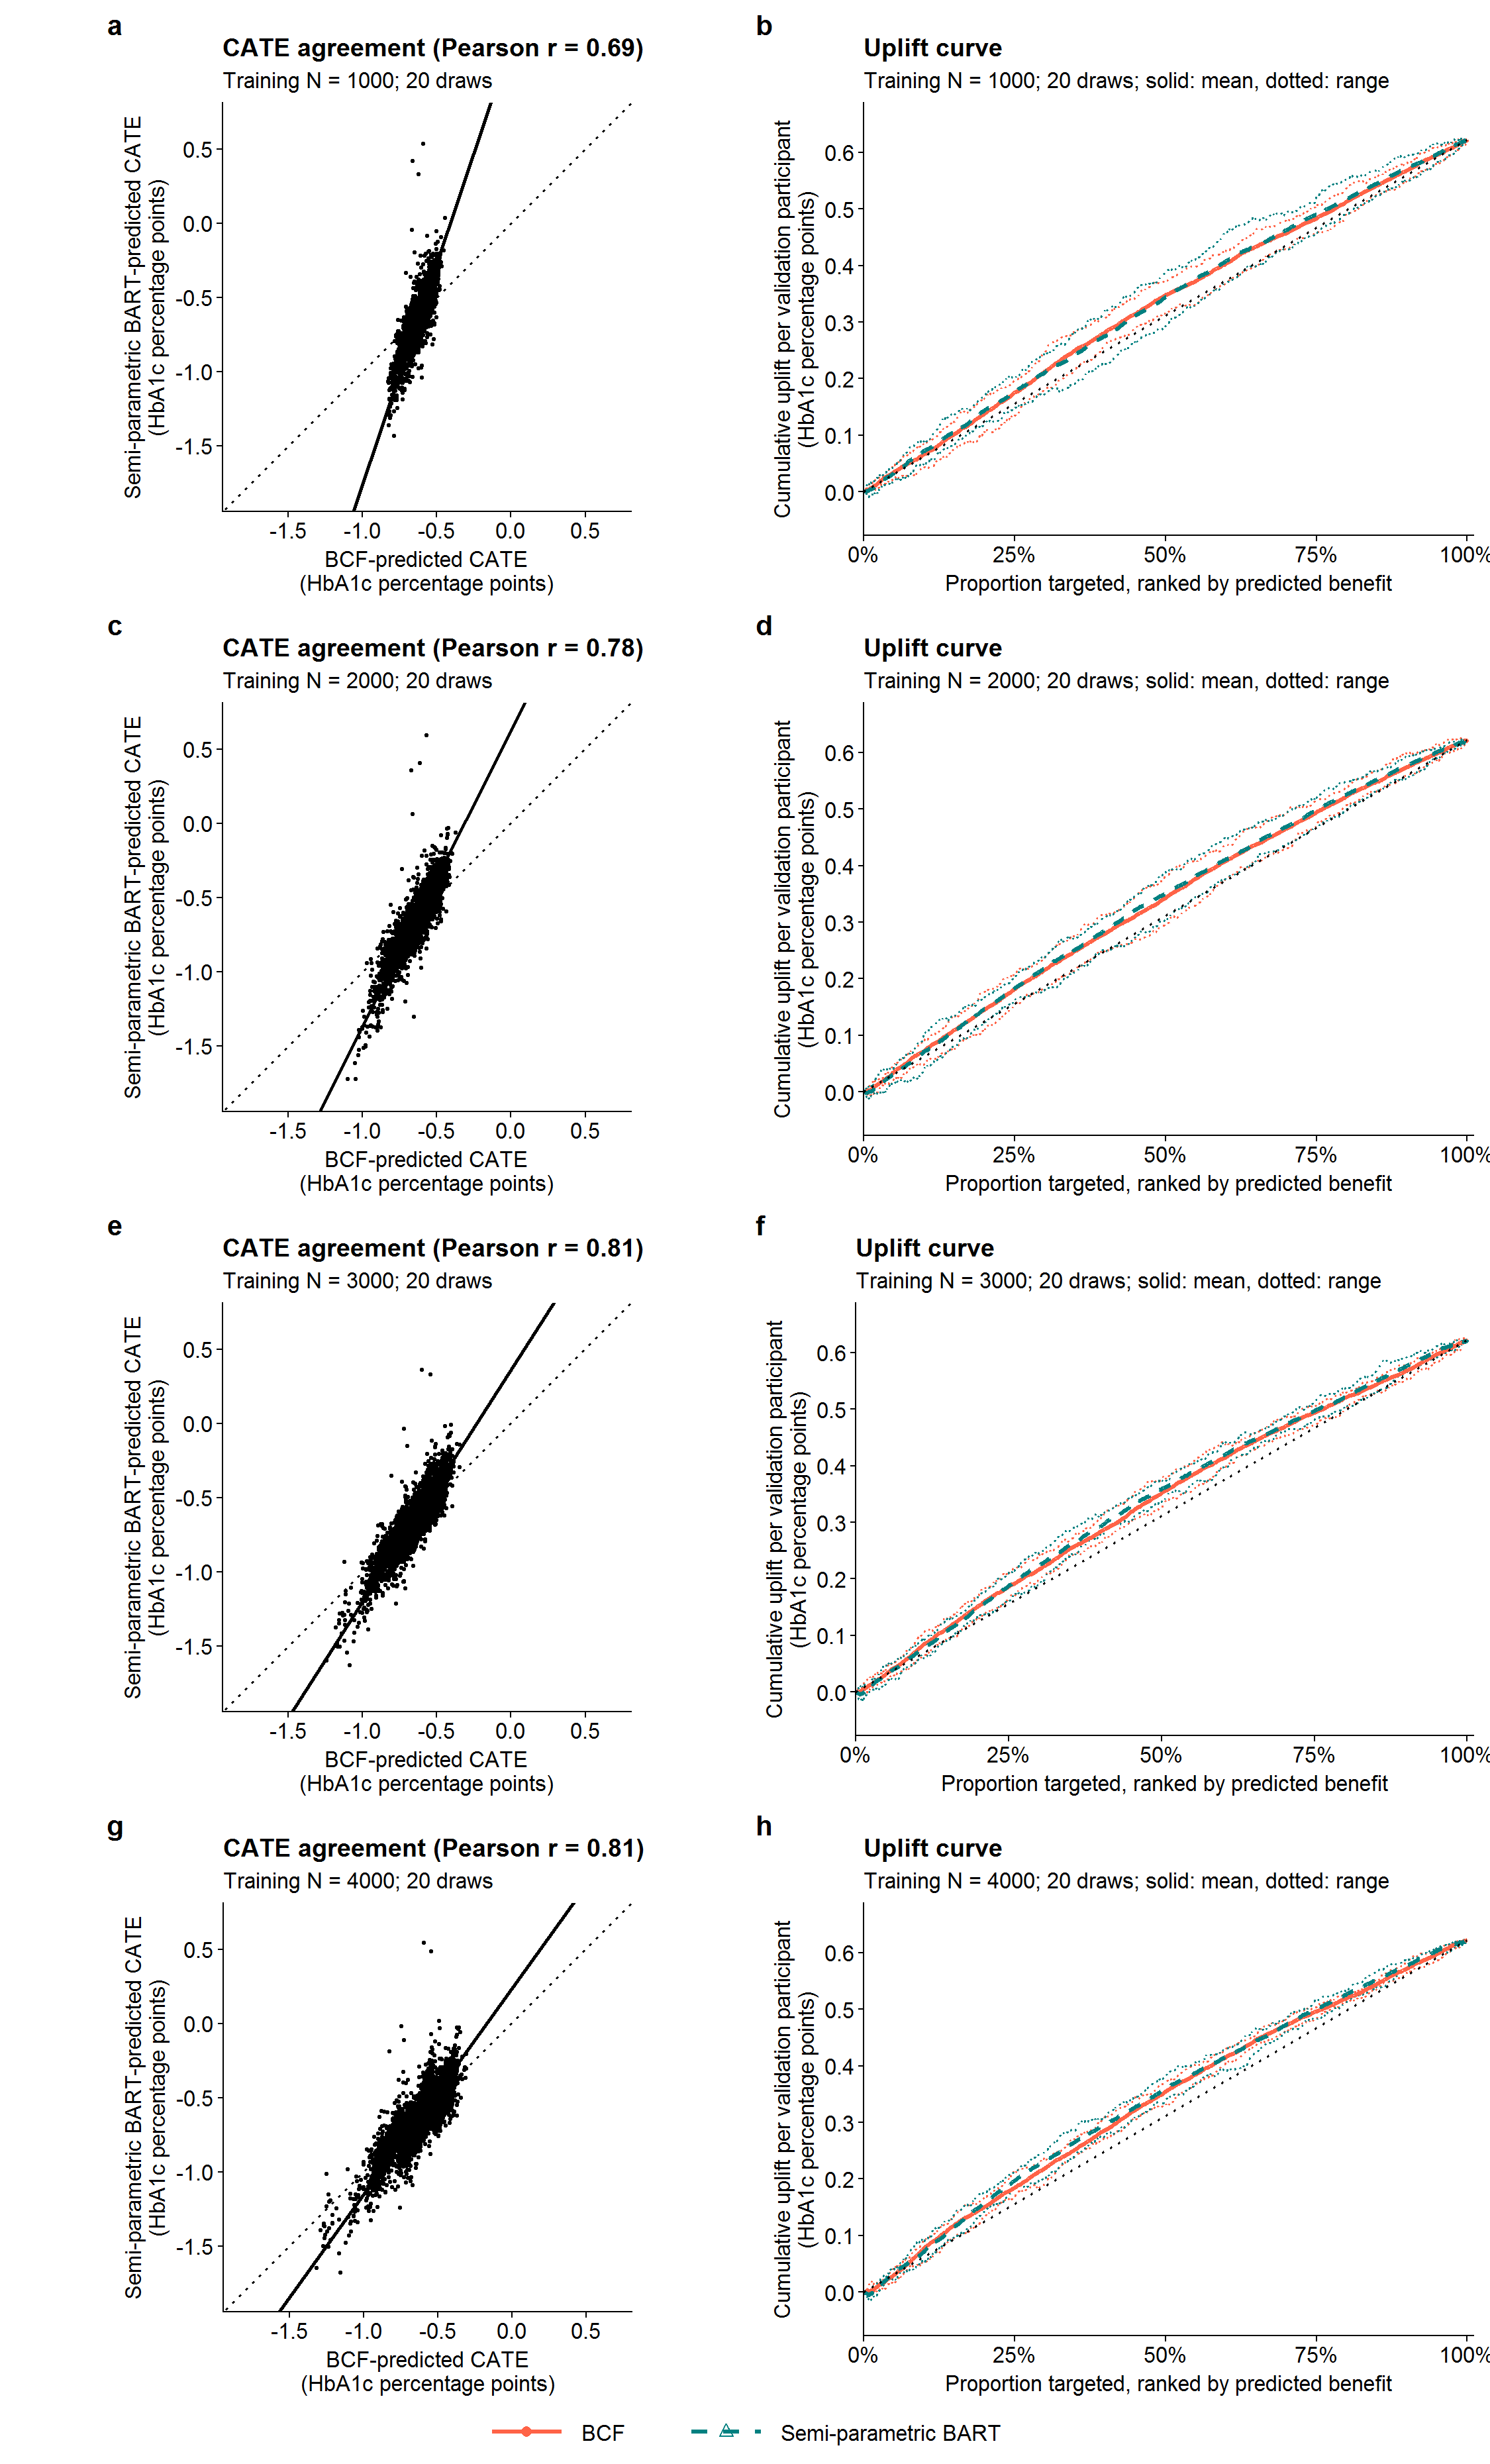
\includegraphics[width=\textwidth,height=0.80\textheight,keepaspectratio]{canvas_hchs_gibbs_20260921_OOS_compound_N1000-2000-3000-4000.png}
    \caption{Out-of-sample CATE agreement (left) and uplift curves (right) for \rev{SP-BART} and BCF at $N=1000$, $2000$, $3000$, and $4000$ (mean over 20 draws). The orthogonal fit is a total least-squares line between the two models' predictions, minimizing perpendicular distances; it is unrelated to treatment residualisation in Section \ref{subsec:ortho_supp}. Dotted min--max lines show the pointwise range across the 20 training draws. The dotted diagonal marks equality in the agreement panels and random targeting in the uplift panels.}
    \label{fig:cv_dashboards}
\end{figure}

\begin{table}[htbp]
\centering
\caption{Out-of-sample performance on CANVAS. Values are mean $\pm$ standard deviation over 20 training draws, except the last row, which is a single fit on the full CANVAS-R sample. RMSE is for the outcome $Y$. Correlation and Spearman are between the two models' out-of-sample CATEs. Net AUUC subtracts the random-targeting area and is divided by the 3004 validation participants; its units are HbA1c change.}
\label{tab:model_metrics}
\resizebox{\textwidth}{!}{%
\begin{tabular}{lccccccc}
\toprule
& & \multicolumn{2}{c}{Outcome RMSE} & \multicolumn{2}{c}{CATE agreement} & \multicolumn{2}{c}{Net AUUC/$n_v$}\\
\cmidrule(lr){3-4}\cmidrule(lr){5-6}\cmidrule(lr){7-8}
$N$ & Draws & BCF & \rev{SP-BART} & $r$ & Spearman & BCF & \rev{SP-BART}\\
\midrule
500 & 20 & $1.009 \pm 0.119$ & $0.947 \pm 0.016$ & $0.702 \pm 0.137$ & $0.759 \pm 0.088$ & $0.009 \pm 0.013$ & $0.012 \pm 0.015$ \\
1000 & 20 & $0.974 \pm 0.078$ & $0.926 \pm 0.009$ & $0.692 \pm 0.130$ & $0.727 \pm 0.108$ & $0.019 \pm 0.010$ & $0.021 \pm 0.014$ \\
1500 & 20 & $0.952 \pm 0.057$ & $0.918 \pm 0.004$ & $0.741 \pm 0.102$ & $0.778 \pm 0.090$ & $0.020 \pm 0.009$ & $0.025 \pm 0.008$ \\
2000 & 20 & $0.979 \pm 0.044$ & $0.916 \pm 0.005$ & $0.778 \pm 0.088$ & $0.803 \pm 0.074$ & $0.023 \pm 0.009$ & $0.026 \pm 0.010$ \\
3000 & 20 & $0.970 \pm 0.058$ & $0.913 \pm 0.002$ & $0.811 \pm 0.069$ & $0.828 \pm 0.052$ & $0.025 \pm 0.004$ & $0.028 \pm 0.006$ \\
4000 & 20 & $0.944 \pm 0.024$ & $0.910 \pm 0.002$ & $0.813 \pm 0.033$ & $0.823 \pm 0.031$ & $0.027 \pm 0.003$ & $0.031 \pm 0.005$ \\
5018 & 1 & $0.950$ & $0.909$ & $0.843$ & $0.851$ & $0.029$ & $0.035$ \\
\bottomrule
\end{tabular}}
\end{table}
\newpage

\subsection{Interpretability and Variable Selection in Practice}
\label{subsec:applied_interpretability}
The out-of-sample evaluations show comparable ranking for the two models. \rev{SP-BART} also allows structural interpretation. We therefore applied the Shapley value decomposition to the CANVAS-R data to describe the covariate contributions to treatment effect heterogeneity. The Shapley summaries and the HbA1c and age coefficient posteriors are shown in the main text (Figures \ref{fig:shapley_contribution} and \ref{fig:posterior_HBA1C}). Table \ref{tab:canvas_covariates} defines the abbreviations.

\begin{table}[htbp]
\centering\small
\caption{Baseline covariates in the CANVAS analysis and figure labels.}
\label{tab:canvas_covariates}
\begin{tabular}{lp{0.73\textwidth}}
\toprule
Label & Covariate\\
\midrule
BLBMI & Body mass index\\
AGE & Age\\
HHFFL & History of heart failure\\
BLSBP & Systolic blood pressure\\
SEX & Sex\\
DIADUR & Diabetes duration\\
HCEREBFL & History of cerebrovascular disease\\
BLA1C & HbA1c\\
BLGFR & Estimated glomerular filtration rate\\
INSULBL & Insulin use\\
GLP1BL & GLP-1 receptor agonist use\\
BLACR & Urinary albumin-to-creatinine ratio\\
RACE & Recorded race, represented by sum contrasts RACE1--RACE5\\
METFORBL & Metformin use\\
RANGIBL & Use of agents acting on the renin--angiotensin system\\
\bottomrule
\end{tabular}
\end{table}

For RACE, the signed column contributions are summed within each individual before taking absolute values. RACE, baseline HbA1c, and age have the largest contributions, predominantly through main effects. The recorded race categories are White; Black or African American; Asian; American Indian or Alaska Native; Native Hawaiian or Other Pacific Islander; and Other/Multiple. We combine Other and Multiple, and treat Unknown and Not Reported as missing before complete-case filtering.

To assess each covariate, we compare the full fitted CATE, including its interactions, at selected values while averaging over the empirical distribution of the other covariates. For continuous covariates, we compare the 90th and 10th percentiles; for binary covariates, the two levels; and for RACE, every pair of categories. For posterior contrast draws $d_\ell^{(m)}$, with posterior mean $\bar d_\ell$ and standard deviation $s_\ell$, we take the $95$th percentile $k$ of $\max_\ell |(d_\ell^{(m)}-\bar d_\ell)/s_\ell|$. The intervals $\bar d_\ell\pm k s_\ell$ are simultaneous across all assessed contrasts. A covariate is flagged when at least one of its intervals excludes zero.

\rev{Figure \ref{fig:canvas_full_contrasts} shows the simultaneous intervals for all assessed contrasts.}

\begin{figure}[p]
    \centering
    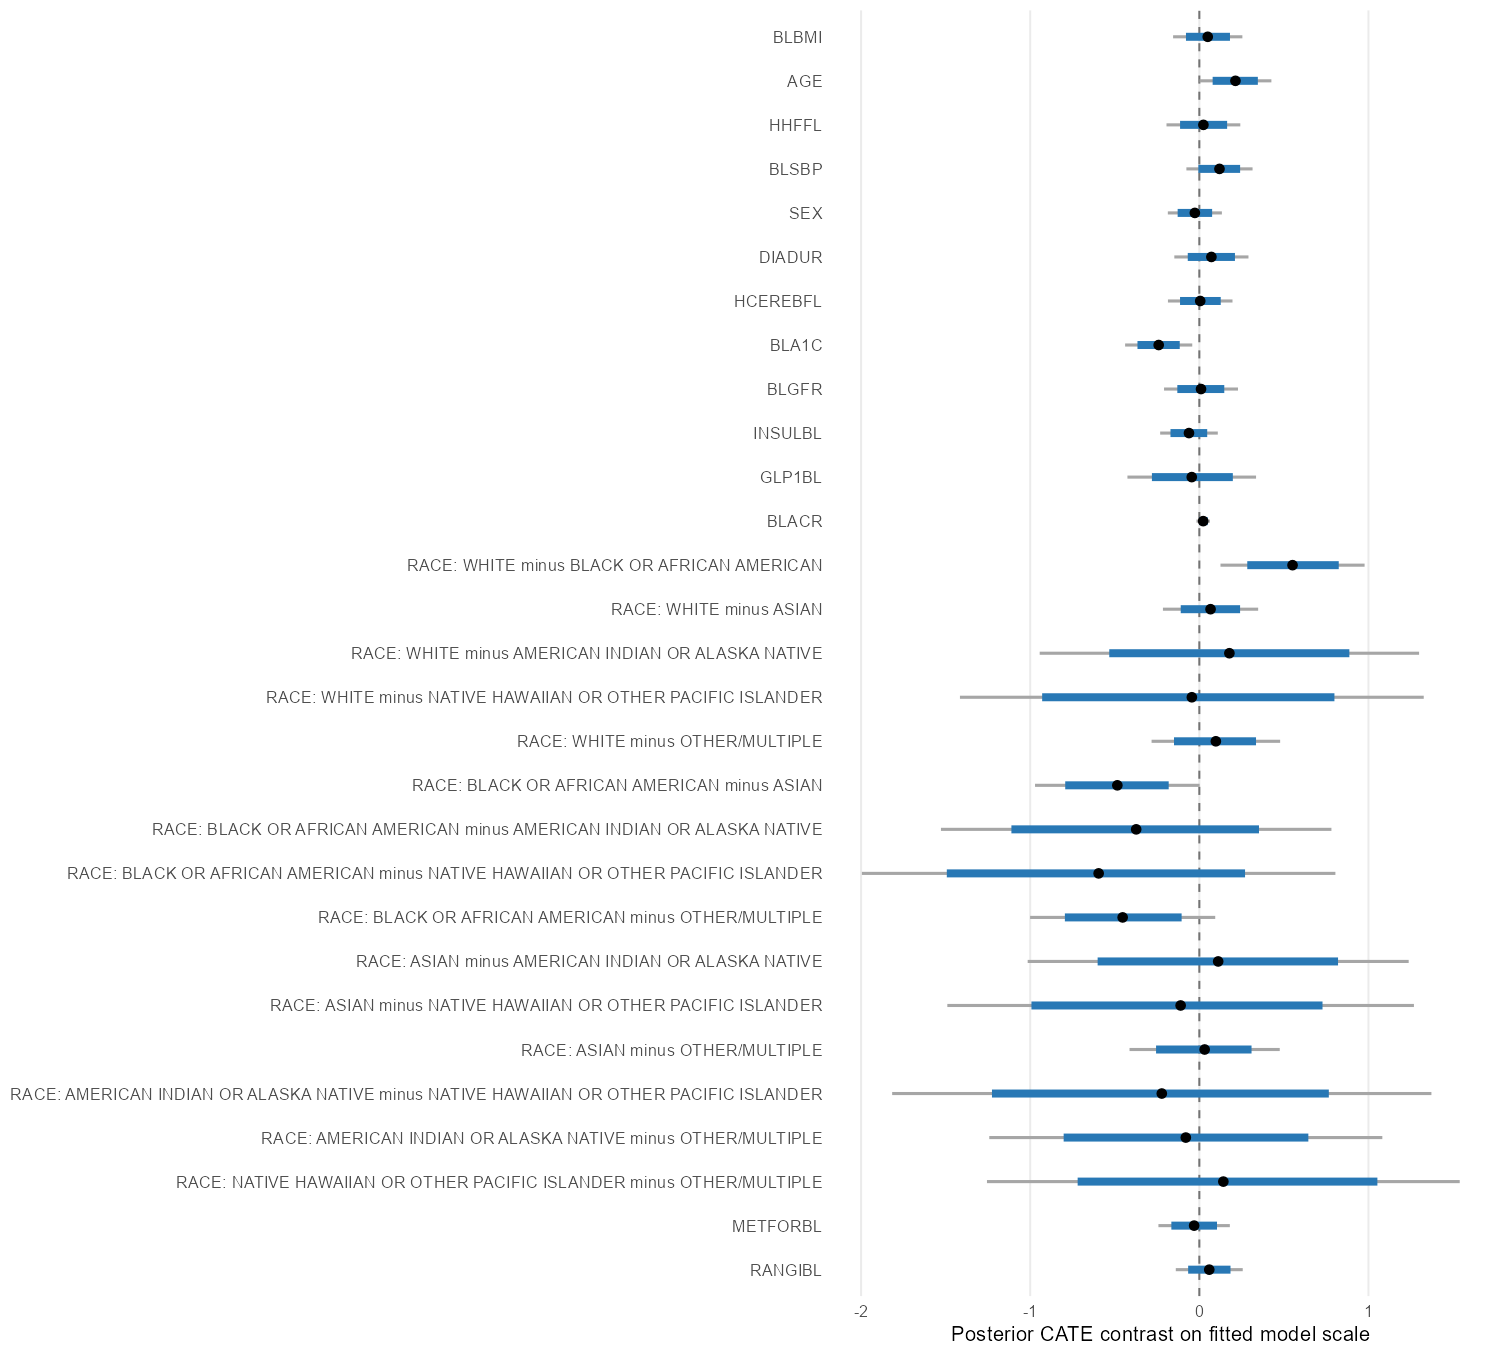
\includegraphics[width=\textwidth,height=0.78\textheight,keepaspectratio]{all_covariate_contrasts.png}
    \caption{\rev{Full fitted CATE contrasts in CANVAS-R, including interactions and averaged over the other covariates. Continuous covariates compare the 90th minus 10th percentile; binary covariates compare the higher-coded minus lower-coded level; RACE compares the first named minus second named category. Points are posterior means; blue and grey intervals are pointwise and simultaneous $95\%$ credible intervals, respectively. Contrasts are on the fitted model scale.}}
    \label{fig:canvas_full_contrasts}
\end{figure}
\FloatBarrier

\section{Ranking Performance in Simulation}
\label{subsec:ranking_supp}

Tables \ref{tab:med_ranking} and \ref{tab:mild_ranking} display interval-based selection performance under the Heavy Saturation and Mild Saturation scenarios, respectively.

Two patterns hold across both scenarios. The advantage of \rev{SP-BART} is concentrated at the sharp thresholds. Under heavy saturation it attains both higher sensitivity and higher precision than BCF at the top 10\% threshold, recovering on average 33.8\% of the true top decile against 3.6\% for BCF, at a mean precision of 0.991 against 0.743. At the top 50\% threshold under heavy saturation, mean sensitivities are similar (0.725 for BCF against 0.722), while their mean precisions are close (0.997 against 0.996). The advantage under this selection rule is therefore concentrated at the more selective threshold.

Table \ref{tab:med_ranking} shows that under heavy saturation the precision of \rev{SP-BART} stays at or above 0.957 at every sample size and threshold, while BCF's top 10\% precision ranges from 0.468 to 0.920 and is weakest when $\mu(x)$ is non-linear. The selection rule can therefore identify high-benefit individuals in this monotone simulation, even though the CATE magnitudes are biased and coverage drops (Table \ref{tab:med_sat_scenario}). Under mild saturation (Table \ref{tab:mild_ranking}) the same ordering shows up from $N \ge 1000$ onwards, but at $N = 250$ neither model is dependable at the top decile: precision falls to 0.615 for \rev{SP-BART} under a linear $\mu(x)$ and to 0.230 for BCF under a non-linear one. At small sample sizes, precision at the sharpest threshold is not stable. These ranking results are for a monotone treatment function.

\begin{table}[ht]
\centering
\caption{Interval-based selection performance: heavy saturation scenario. A patient is flagged if the lower bound of the 95\% credible interval exceeds the threshold. Precision is averaged only over replicates in which the model flagged at least one patient, so it should be read together with sensitivity.}
\label{tab:med_ranking}
\resizebox{\textwidth}{!}{
\begin{tabular}{lr cc cc cc c cc cc cc}
\toprule
& & \multicolumn{6}{c}{\textbf{ BCF}} & & \multicolumn{6}{c}{\textbf{\rev{SP-BART}}} \\
\cmidrule{3-8} \cmidrule{10-15}
$\mu(x)$ Form & $N$ & \multicolumn{2}{c}{Top 10\%} & \multicolumn{2}{c}{Top 25\%} & \multicolumn{2}{c}{Top 50\%} & & \multicolumn{2}{c}{Top 10\%} & \multicolumn{2}{c}{Top 25\%} & \multicolumn{2}{c}{Top 50\%} \\
\cmidrule{3-4} \cmidrule{5-6} \cmidrule{7-8} \cmidrule{10-11} \cmidrule{12-13} \cmidrule{14-15}
& & Sens & Prec & Sens & Prec & Sens & Prec & & Sens & Prec & Sens & Prec & Sens & Prec \\
\midrule
\multirow{6}{*}{Linear}
& 250 & 0.060 & 0.797 & 0.095 & 0.961 & 0.510 & 0.994 &  & 0.167 & 0.965 & 0.159 & 0.994 & 0.512 & 0.987 \\
& 500 & 0.060 & 0.870 & 0.147 & 0.993 & 0.666 & 0.999 &  & 0.251 & 0.992 & 0.237 & 1.000 & 0.675 & 0.996 \\
& 750 & 0.068 & 0.883 & 0.190 & 0.990 & 0.726 & 0.999 &  & 0.315 & 0.996 & 0.282 & 1.000 & 0.729 & 0.997 \\
& 1000 & 0.064 & 0.907 & 0.219 & 0.995 & 0.760 & 0.999 &  & 0.356 & 0.999 & 0.316 & 1.000 & 0.774 & 0.998 \\
& 1500 & 0.056 & 0.897 & 0.297 & 0.994 & 0.807 & 0.998 &  & 0.410 & 1.000 & 0.356 & 1.000 & 0.810 & 0.998 \\
& 3000 & 0.047 & 0.920 & 0.519 & 0.994 & 0.856 & 0.999 &  & 0.515 & 1.000 & 0.422 & 1.000 & 0.866 & 0.999 \\
\midrule
\multirow{6}{*}{Non-linear}
& 250 & 0.017 & 0.468 & 0.043 & 0.852 & 0.505 & 0.992 &  & 0.172 & 0.957 & 0.162 & 0.986 & 0.517 & 0.990 \\
& 500 & 0.015 & 0.560 & 0.092 & 0.927 & 0.696 & 0.997 &  & 0.266 & 0.990 & 0.252 & 0.999 & 0.661 & 0.996 \\
& 750 & 0.009 & 0.623 & 0.118 & 0.975 & 0.733 & 0.998 &  & 0.318 & 0.999 & 0.284 & 1.000 & 0.715 & 0.999 \\
& 1000 & 0.010 & 0.552 & 0.179 & 0.980 & 0.766 & 0.998 &  & 0.354 & 0.998 & 0.314 & 1.000 & 0.752 & 0.999 \\
& 1500 & 0.009 & 0.654 & 0.305 & 0.992 & 0.819 & 0.999 &  & 0.424 & 1.000 & 0.362 & 1.000 & 0.800 & 0.999 \\
& 3000 & 0.016 & 0.784 & 0.516 & 0.998 & 0.862 & 0.998 &  & 0.509 & 1.000 & 0.418 & 1.000 & 0.857 & 0.999 \\
\bottomrule
\end{tabular}}
\end{table}

\begin{table}[ht]
\centering
\caption{Interval-based selection performance: mild saturation scenario. A patient is flagged if the lower bound of the 95\% credible interval exceeds the threshold. Precision is averaged only over replicates in which the model flagged at least one patient, so it should be read together with sensitivity.}
\label{tab:mild_ranking}
\resizebox{\textwidth}{!}{
\begin{tabular}{lr cc cc cc c cc cc cc}
\toprule
& & \multicolumn{6}{c}{\textbf{BCF}} & & \multicolumn{6}{c}{\textbf{\rev{SP-BART}}} \\
\cmidrule{3-8} \cmidrule{10-15}
$\mu(x)$ Form & $N$ & \multicolumn{2}{c}{Top 10\%} & \multicolumn{2}{c}{Top 25\%} & \multicolumn{2}{c}{Top 50\%} & & \multicolumn{2}{c}{Top 10\%} & \multicolumn{2}{c}{Top 25\%} & \multicolumn{2}{c}{Top 50\%} \\
\cmidrule{3-4} \cmidrule{5-6} \cmidrule{7-8} \cmidrule{10-11} \cmidrule{12-13} \cmidrule{14-15}
& & Sens & Prec & Sens & Prec & Sens & Prec & & Sens & Prec & Sens & Prec & Sens & Prec \\
\midrule
\multirow{6}{*}{Linear}
& 250 & 0.045 & 0.648 & 0.049 & 0.790 & 0.071 & 0.893 &  & 0.064 & 0.615 & 0.080 & 0.719 & 0.129 & 0.865 \\
& 500 & 0.052 & 0.880 & 0.061 & 0.962 & 0.109 & 0.972 &  & 0.071 & 0.823 & 0.105 & 0.920 & 0.192 & 0.967 \\
& 750 & 0.064 & 0.883 & 0.075 & 0.955 & 0.136 & 0.984 &  & 0.098 & 0.897 & 0.142 & 0.953 & 0.252 & 0.982 \\
& 1000 & 0.067 & 0.921 & 0.090 & 0.962 & 0.163 & 0.986 &  & 0.088 & 0.957 & 0.157 & 0.979 & 0.309 & 0.986 \\
& 1500 & 0.066 & 0.915 & 0.110 & 0.973 & 0.233 & 0.992 &  & 0.112 & 0.980 & 0.209 & 0.986 & 0.392 & 0.992 \\
& 3000 & 0.090 & 0.960 & 0.207 & 0.987 & 0.425 & 0.996 &  & 0.234 & 0.991 & 0.366 & 0.994 & 0.568 & 0.995 \\
\midrule
\multirow{6}{*}{Non-linear}
& 250 & 0.010 & 0.230 & 0.018 & 0.492 & 0.039 & 0.765 &  & 0.054 & 0.568 & 0.064 & 0.752 & 0.108 & 0.902 \\
& 500 & 0.012 & 0.298 & 0.021 & 0.617 & 0.068 & 0.869 &  & 0.068 & 0.832 & 0.107 & 0.927 & 0.186 & 0.972 \\
& 750 & 0.005 & 0.411 & 0.023 & 0.763 & 0.086 & 0.935 &  & 0.081 & 0.943 & 0.125 & 0.977 & 0.232 & 0.990 \\
& 1000 & 0.009 & 0.445 & 0.032 & 0.835 & 0.145 & 0.963 &  & 0.089 & 0.965 & 0.154 & 0.986 & 0.294 & 0.994 \\
& 1500 & 0.016 & 0.590 & 0.066 & 0.906 & 0.235 & 0.984 &  & 0.144 & 0.984 & 0.235 & 0.991 & 0.400 & 0.996 \\
& 3000 & 0.035 & 0.762 & 0.159 & 0.982 & 0.439 & 0.996 &  & 0.243 & 0.994 & 0.371 & 0.997 & 0.555 & 0.998 \\
\bottomrule
\end{tabular}}
\end{table}




\FloatBarrier
\section{Computational Details}
\label{sec:full_conditionals}
\label{sec:computational_details}

We use Bayesian backfitting to alternate between the prognostic and treatment
functions. Let $u_i$ denote the fixed treatment coding, with $u_i=z_i$ for
$0/1$ coding and $u_i=z_i-1/2$ for symmetric coding. Let $h_i$ contain the
$p$ covariate columns and the $q$ included interaction columns, and collect
their coefficients in $b$. The treatment-weighted design $W$ has rows
$u_i h_i^\top$, so that $y=\mu+u\alpha+Wb+\varepsilon$ and
$\tau(x_i)=\alpha+h_i^\top b$. Write $\mathcal P$ for the included interaction pairs, $K=p+q$, and
\[
 D=\operatorname{diag}\left(\lambda_1^2,\ldots,\lambda_p^2,
       \{\lambda_{j,k}^2\lambda_{\mathrm{glob}}^2\}_{(j,k)\in\mathcal P}\right),
 \qquad Q=W^\top W+D^{-1}.
\]
\rev{All quantities below are on the fitted scale, after centering the outcome and dividing it by its training-sample standard deviation. The simulations use the generated covariates, while IHDP and CANVAS standardize continuous covariates before forming interaction products. Binary and categorical contrast columns and the treatment coding are not standardized.} We use the inverse-gamma
parameterization $p(v)\propto v^{-a-1}\exp(-b/v)$ for
$v\sim\operatorname{IG}(a,b)$; conditioning on the data and all other
current parameters is denoted by $\mid -$.

For the prognostic function, we use the BART prior of
\citet{chipman2010bart}, with $T=250$ trees and splitting probability
$0.95(1+d)^{-2}$ at depth $d$, a maximum depth of 10, and at least five
observations per leaf. Given leaf variance $s_\mu^2$, the leaf parameters
have independent $\mathcal N(0,s_\mu^2)$ priors. For a leaf containing
$n_{t\ell}$ observations, let $S_{t\ell}$ be the sum of the tree-specific
partial residuals defined in Algorithm~\ref{algorithm backfitting}. Then
\begin{equation}
 v_{t\ell}=\left(\frac{n_{t\ell}}{\sigma^2}+\frac{1}{s_\mu^2}\right)^{-1},
 \qquad
 \theta_{t\ell}\mid -\sim
 \mathcal N\left(\frac{v_{t\ell}S_{t\ell}}{\sigma^2},v_{t\ell}\right).
 \label{eq:fc_leaf}
\end{equation}
With $s_\mu^2\sim\operatorname{IG}(a_\mu/2,b_\mu/2)$ and $L$ leaves
across the forest, the leaf variance is drawn from
\begin{equation}
 s_\mu^2\mid -\sim\operatorname{IG}\left(
 \frac{a_\mu+L}{2},\frac{b_\mu+\sum_{t,\ell}\theta_{t\ell}^2}{2}\right),
 \qquad a_\mu=3,\quad b_\mu=1/T.
 \label{eq:fc_leaf_scale}
\end{equation}

The treatment intercept and coefficients have the Gaussian full conditionals
\begin{align}
 v_\alpha&=\left(\frac{u^\top u}{\sigma^2}+\frac{1}{100}\right)^{-1},
 &\alpha\mid -&\sim\mathcal N\left(
 \frac{v_\alpha u^\top(y-\mu-Wb)}{\sigma^2},v_\alpha\right),
 \label{eq:fc_alpha}\\
 b\mid -&\sim\mathcal N_K\left(
 Q^{-1}W^\top(y-\mu-u\alpha),\;\sigma^2Q^{-1}\right).
 \label{eq:fc_beta}
\end{align}
Following \citet{makalic2015simple}, a unit half-Cauchy scale is represented
by $\lambda^2\mid\nu\sim\operatorname{IG}(1/2,1/\nu)$ and
$\nu\sim\operatorname{IG}(1/2,1)$. Applying this to each local scale and
using auxiliary variable $\xi$ for the global scale gives
\begin{align}
 \nu_j\mid -&\sim\operatorname{IG}(1,1+\lambda_j^{-2}),
 &\lambda_j^2\mid -&\sim\operatorname{IG}\left(
 1,\frac{1}{\nu_j}+\frac{\beta_j^2}{2\sigma^2}\right),
 \label{eq:fc_lambda_main}\\
 \nu_{j,k}\mid -&\sim\operatorname{IG}(1,1+\lambda_{j,k}^{-2}),
 &\lambda_{j,k}^2\mid -&\sim\operatorname{IG}\left(
 1,\frac{1}{\nu_{j,k}}+
 \frac{\beta_{j,k}^2}{2\sigma^2\lambda_{\mathrm{glob}}^2}\right),
 \label{eq:fc_lambda_int}\\
 \xi\mid -&\sim\operatorname{IG}(1,1+\lambda_{\mathrm{glob}}^{-2}),
 &\lambda_{\mathrm{glob}}^2\mid -&\sim\operatorname{IG}\left(
 \frac{q+1}{2},\frac{1}{\xi}+\frac{1}{2\sigma^2}
 \sum_{(j,k)\in\mathcal P}\frac{\beta_{j,k}^2}{\lambda_{j,k}^2}\right).
 \label{eq:fc_global}
\end{align}
The main effects have local scales only; the global scale applies to the
interaction block. Finally, with total residuals $e=y-\mu-u\alpha-Wb$,
\begin{equation}
 \sigma^2\mid -\sim\operatorname{IG}\left(
 1+\frac{N+K}{2},\;0.001+\frac{e^\top e+b^\top D^{-1}b}{2}\right).
 \label{eq:fc_sigma}
\end{equation}
The intercept and leaf priors are independent of $\sigma^2$; the
regularized coefficient priors contribute the additional $K/2$ and
$b^\top D^{-1}b/2$ terms.

\begin{algorithm}[htbp]
\caption{Bayesian Backfitting MCMC Scheme for \rev{SP-BART}}
\label{algorithm backfitting}
\begin{algorithmic}[1]
\State \textbf{Initialize:} Prognostic forest $\mu(\cdot)$, leaf variance
$s_\mu^2$, linear parameters $\alpha,b$, local and global shrinkage
parameters, auxiliary variables, and noise variance $\sigma^2$.
\State Fix the covariates, interactions, treatment coding $u$, and propensity
score (fitted in observational data or known from the randomized design).
\For{iteration $m=1,\dots,N_{\mathrm{burn}}+N_{\mathrm{keep}}$}
    \State \textbf{1. Update Prognostic Function ($\mu$):}
    \State Compute partial residuals for $i=1,\ldots,N$:
    \State \quad $R_i^*=y_i-u_i\tau^{(m-1)}(x_i)$.
    \For{each tree $t=1,\ldots,T$}
        \State Compute tree-specific residuals
        $R^*_{i,(-t)}=R_i^*-\sum_{s\ne t}g_s(x_i,\hat\pi_i)$.
        \State Propose a tree modification (e.g., grow, prune) and
        accept/reject via Metropolis--Hastings, integrating out leaf values.
        \State Draw the leaf parameters conditional on the updated tree
        structure and $R^*_{i,(-t)}$ using \eqref{eq:fc_leaf}.
    \EndFor
    \State Draw the common leaf variance using \eqref{eq:fc_leaf_scale}.
    \State \textbf{2. Update Treatment Function ($\tau$):}
    \State Compute partial residuals for $i=1,\ldots,N$:
    \State \quad $R_i^{**}=y_i-\mu^{(m)}(x_i,\hat\pi_i)$.
    \State Draw the intercept $\alpha$ using \eqref{eq:fc_alpha}.
    \State Draw the main-effect and interaction coefficients jointly in $b$
    using \eqref{eq:fc_beta}, with residuals $R^{**}-u\alpha$ and design $W$.
    \State Draw each local auxiliary and then its local scale using
    \eqref{eq:fc_lambda_main} and \eqref{eq:fc_lambda_int}.
    \State Draw the global auxiliary $\xi$ and then
    $\lambda_{\mathrm{glob}}^2$ using \eqref{eq:fc_global}.
    \State Update the CATE function:
    \State \quad $\tau^{(m)}(x_i)=\alpha+\sum_{j=1}^{p}\beta_j x_{i,j}+\sum_{(j,k)\in\mathcal P}\beta_{j,k}x_{i,j}x_{i,k}$.
    \State \textbf{3. Update Noise Variance ($\sigma^2$):}
    \State Compute total residuals:
    \State \quad $e_i=y_i-\mu^{(m)}(x_i,\hat\pi_i)-u_i\tau^{(m)}(x_i)$.
    \State Draw $\sigma^{2(m)}$ using \eqref{eq:fc_sigma}, including the
    coefficient-prior term $b^\top D^{-1}b$.
    \If{$m>N_{\mathrm{burn}}$}
        \State Store the draw and the predictions of interest.
    \EndIf
\EndFor
\end{algorithmic}
\end{algorithm}

The latest available parameter values are used at each step.

\FloatBarrier
\bibliographystyle{apalike}
\bibliography{references-8.3.5}
\end{document}
